%
% $RCSfile: project.tex,v $
%
% Copyright (C) 2002-2008. Christian Heller.
%
% Permission is granted to copy, distribute and/or modify this document
% under the terms of the GNU Free Documentation License, Version 1.1 or
% any later version published by the Free Software Foundation; with no
% Invariant Sections, with no Front-Cover Texts and with no Back-Cover
% Texts. A copy of the license is included in the section entitled
% "GNU Free Documentation License".
%
% http://www.cybop.net
% - Cybernetics Oriented Programming -
%
% http://www.resmedicinae.org
% - Information in Medicine -
%
% Version: $Revision: 1.1 $ $Date: 2008-08-19 20:41:08 $ $Author: christian $
% Authors: Christian Heller <christian.heller@tuxtax.de>
%

\section{Project}
\label{project_heading}
\index{Res Medicinae Project}
\index{Hospital Information System}
\index{HIS}
\index{Practice Management System}
\index{PMS}
\index{Electronic Health Record}
\index{EHR}

The -- somewhat idealistic -- aim was initially to create the prototype of a
\emph{Hospital Information System} (HIS). Due to the clearly too high-set aims,
this was later revised so that the focus of the prototype became a standard
\emph{Practice Management System} (PMS) with an \emph{Electronic Health Record}
(EHR) as its core. Several technology changes during the progress of this work
and the lack in time required to also revise this aim, so that now the final
prototype consists of just the (rudimentary) address management module of the
planned EHR application. It is written in CYBOL and executable by CYBOI.

The following sections describe the project background of \emph{Res Medicinae}.

%
% $RCSfile: free_and_open_source_software.tex,v $
%
% Copyright (C) 2002-2008. Christian Heller.
%
% Permission is granted to copy, distribute and/or modify this document
% under the terms of the GNU Free Documentation License, Version 1.1 or
% any later version published by the Free Software Foundation; with no
% Invariant Sections, with no Front-Cover Texts and with no Back-Cover
% Texts. A copy of the license is included in the section entitled
% "GNU Free Documentation License".
%
% http://www.cybop.net
% - Cybernetics Oriented Programming -
%
% http://www.resmedicinae.org
% - Information in Medicine -
%
% Version: $Revision: 1.1 $ $Date: 2008-08-19 20:41:06 $ $Author: christian $
% Authors: Christian Heller <christian.heller@tuxtax.de>
%

\subsection{Free and Open Source Software}
\label{free_and_open_source_software_heading}
\index{Free and Open Source Software}
\index{FOSS}
\index{Free/ Libre Open Source Software}
\index{FLOSS}
\index{General Public License}
\index{GPL}
\index{Free Documentation License}
\index{FDL}
\index{Open Source Software}
\index{OSS}

Just like CYBOP (including CYBOL and CYBOI) \cite{cybop}, \emph{Res Medicinae}
\cite{resmedicinae} is developed within a \emph{Free/ Libre Open Source Software}
(FLOSS) project. Its source code, resources and documentation are placed under
GNU's \emph{General Public License} (GPL) (section
\ref{gnu_general_public_license_heading}) and \emph{Free Documentation License}
(FDL) (section \ref{gnu_free_documentation_license_heading}), respectively.
That means they can be freely redistributed and modified under the terms of
these licences. Although distributed in the hope that they will be useful, the
program and its resources come \emph{without any warranty}, without even the
implied warranty of \emph{merchantability or fitness for a particular purpose}.
See \cite{gnulicences} for details.

More information on \emph{Open Source Software} (OSS) in general can be found
at \cite{opensource}. There are plenty of resources for further background
reading, a German one being the \emph{Open Source Jahrbuch 2004}
\cite{opensourcejahrbuch2004}. To what concerns FLOSS in the medical arena,
many other projects exist. Comprehensive lists of these can be found at
\cite{euspirit, linuxmednews, medhowto}.

%
% $RCSfile: portals_and_services.tex,v $
%
% Copyright (C) 2002-2008. Christian Heller.
%
% Permission is granted to copy, distribute and/or modify this document
% under the terms of the GNU Free Documentation License, Version 1.1 or
% any later version published by the Free Software Foundation; with no
% Invariant Sections, with no Front-Cover Texts and with no Back-Cover
% Texts. A copy of the license is included in the section entitled
% "GNU Free Documentation License".
%
% http://www.cybop.net
% - Cybernetics Oriented Programming -
%
% http://www.resmedicinae.org
% - Information in Medicine -
%
% Version: $Revision: 1.1 $ $Date: 2008-08-19 20:41:08 $ $Author: christian $
% Authors: Christian Heller <christian.heller@tuxtax.de>
%

\subsection{Portals and Services}
\label{portals_and_services_heading}
\index{Open Source Development Portals and Services}
\index{Sourceforge Development Portal}
\index{Freshmeat Development Portal}
\index{BerliOS Development Portal}
\index{Savannah Development Portal}
\index{Free Software Foundation}
\index{FSF}

As OSS became popular over the years, the number of its supporters rose. It is
not long time that \emph{Sourceforge} \cite{sourceforge}, the first
\emph{Development Portal} for FLOSS, was opened. Shortly after, others like
\emph{Freshmeat} \cite{freshmeat} followed and meanwhile, there are also
national initiatives like \emph{BerliOS} \cite{berlios} in Germany. Also the
\emph{Free Software Foundation} (FSF) offers an own portal called
\emph{Savannah} \cite{savannah}, hosting exclusively \emph{free} \cite{gnu}
software projects. Figure \ref{portals_figure} shows the four portals by their
name, logo and \emph{Uniform Resource Locator} (URL).

\begin{figure}[ht]
    \begin{center}
        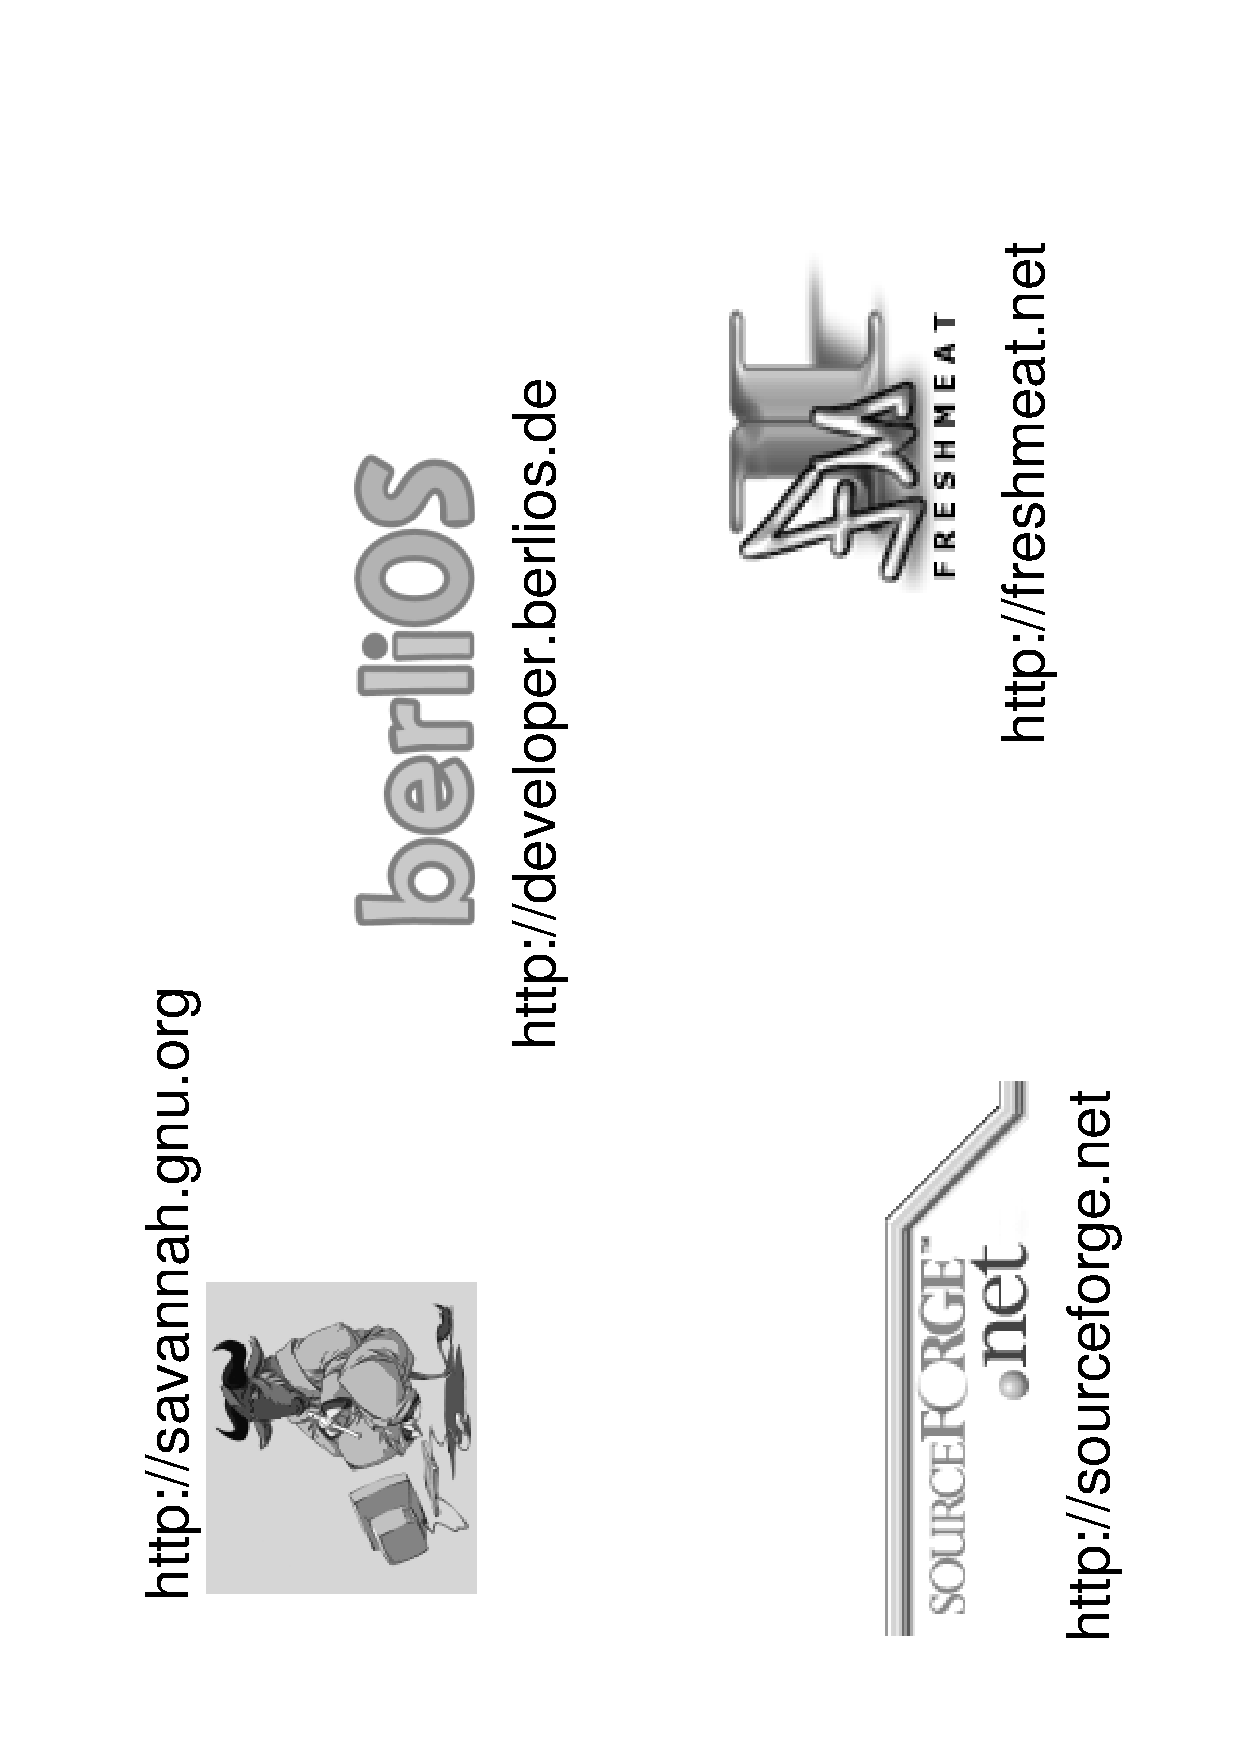
\includegraphics[scale=0.3,angle=-90]{graphic/portals.pdf}
        \caption{FLOSS Development Portals}
        \label{portals_figure}
    \end{center}
\end{figure}

As \emph{BerliOS} states in its slogan, it is the aim of development portals of
that kind to \textit{foster open source development}. In \emph{Savannah's}
words, they are \textit{central points for the development, distribution and
maintenance of FLOSS}. Although very often supported by well-known sponsors,
most portals are and want to stay independent. Using them, OSS projects and their
developers are offered several free services (figure \ref{services_figure}).
Since not all of these are always useful, projects can configure their portal
sites as needed.

\begin{figure}[ht]
    \begin{center}
        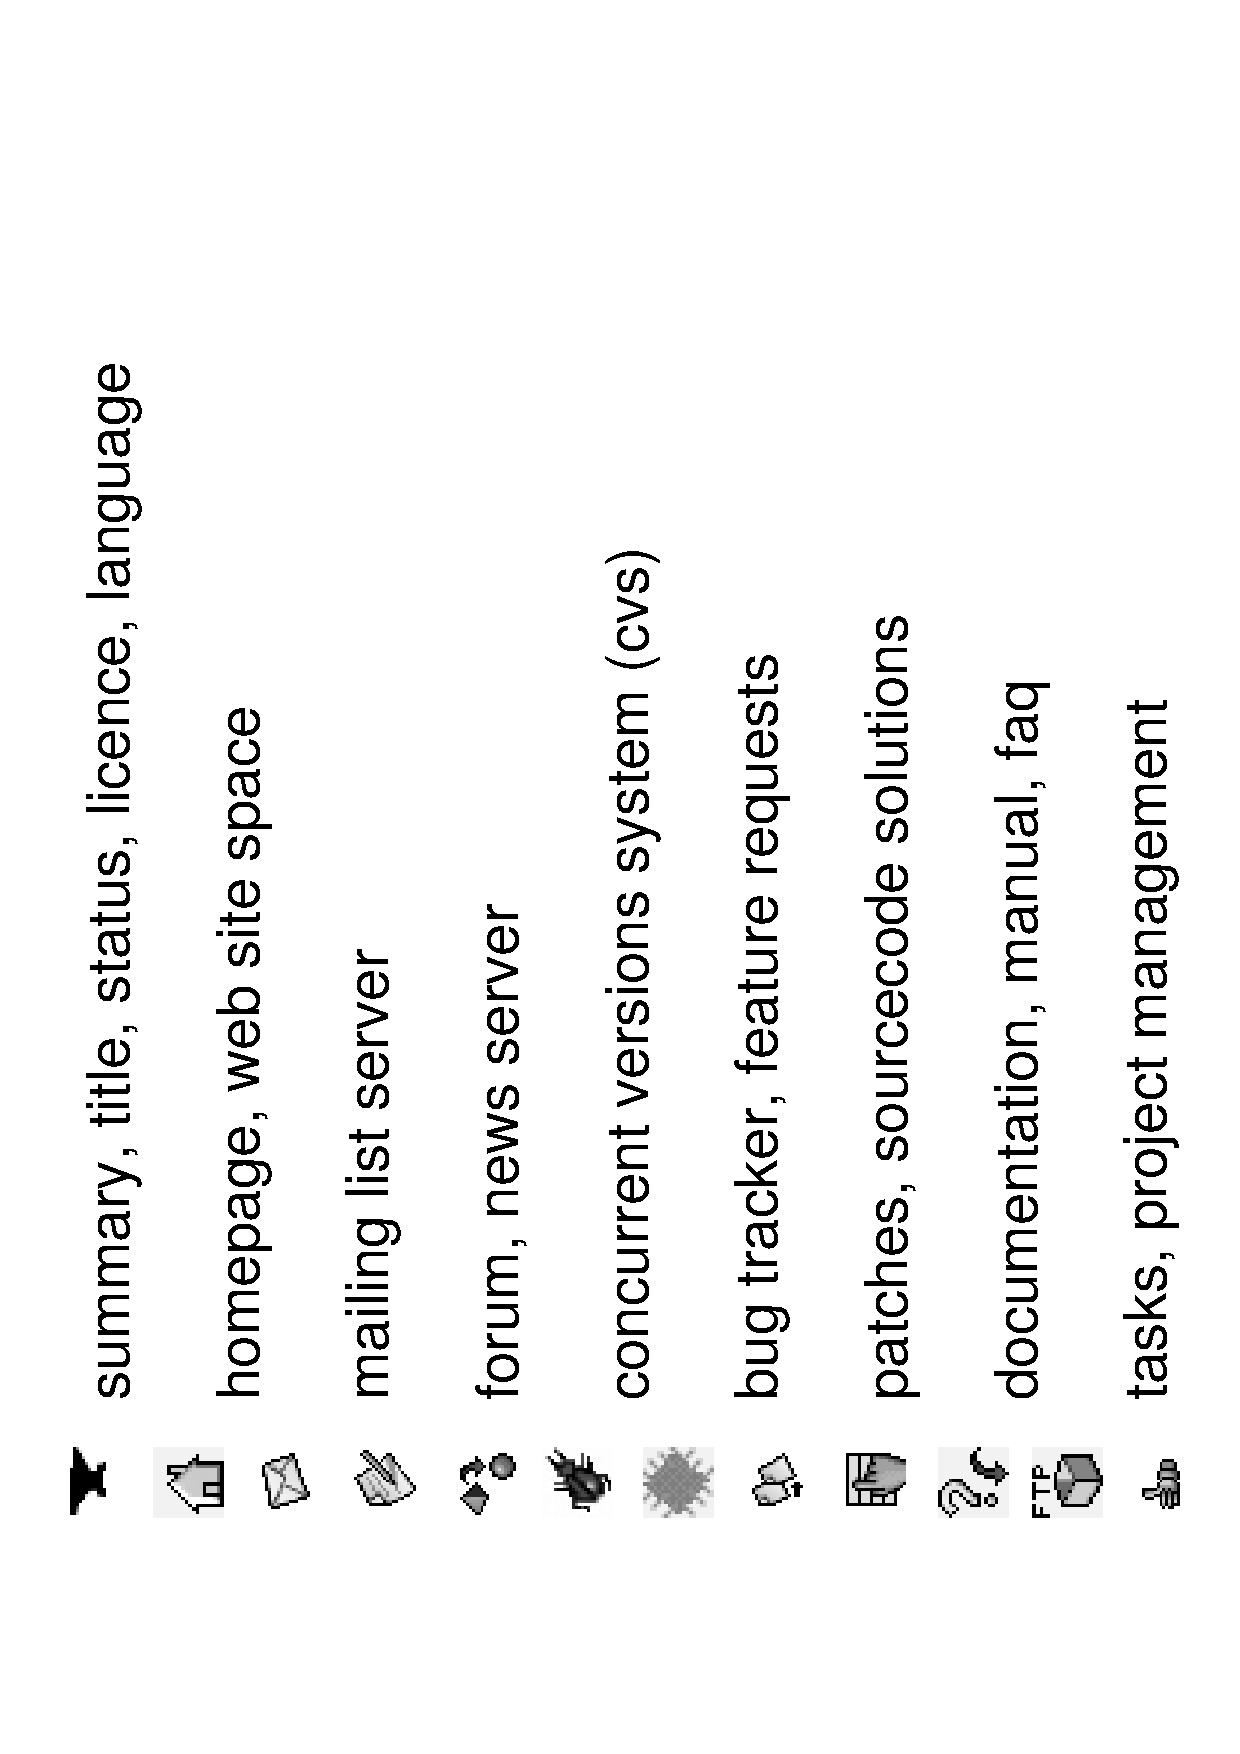
\includegraphics[scale=0.3,angle=-90]{graphic/services.pdf}
        \caption{Portal Services}
        \label{services_figure}
    \end{center}
\end{figure}

\emph{Res Medicinae} was one of the first OSS projects registered at
Sourceforge (number 4237 of now more than 100,000). CYBOP (CYBOL, CYBOI) is
hosted at BerliOS.

%
% $RCSfile: tools.tex,v $
%
% Copyright (C) 2002-2008. Christian Heller.
%
% Permission is granted to copy, distribute and/or modify this document
% under the terms of the GNU Free Documentation License, Version 1.1 or
% any later version published by the Free Software Foundation; with no
% Invariant Sections, with no Front-Cover Texts and with no Back-Cover
% Texts. A copy of the license is included in the section entitled
% "GNU Free Documentation License".
%
% http://www.cybop.net
% - Cybernetics Oriented Programming -
%
% http://www.resmedicinae.org
% - Information in Medicine -
%
% Version: $Revision: 1.1 $ $Date: 2008-08-19 20:41:09 $ $Author: christian $
% Authors: Christian Heller <christian.heller@tuxtax.de>
%

\subsection{Tools}
\label{tools_heading}
\index{Res Medicinae Development Tools}

Classical application development relies on tools like a \emph{UML Designer}, for
creating \emph{Unified Modeling Language} (UML) diagrams, a \emph{Text Editor},
\emph{Compiler} and \emph{Debugger}. Nowadays, these and other tools are
offered in one package, as \emph{Integrated Development Environment} (IDE).

Because the CYBOI interpreter is written in the system programming language
\emph{C}, its development requires a compiler. CYBOL applications, on the other
hand, do not have to be compiled. They base on interpreted XML code which can
be written in every text editor; nothing else is needed. An adapted editor was
proposed in section \ref{template_editor_heading}.

Res Medicinae development could certainly be speeded up by using graphical
diagrams in the style of the UML. But unfortunately, design tools that directly
support CYBOP do not exist yet. As section \ref{knowledge_designer_heading}
tried to show, some UML diagrams could be used with only minor adaptations for
CYBOL modelling. For the time being, standard XML editors have to suffice.

For running and testing CYBOL applications, of course, the CYBOI interpreter is
needed.

%
% $RCSfile: contributors.tex,v $
%
% Copyright (C) 2002-2008. Christian Heller.
%
% Permission is granted to copy, distribute and/or modify this document
% under the terms of the GNU Free Documentation License, Version 1.1 or
% any later version published by the Free Software Foundation; with no
% Invariant Sections, with no Front-Cover Texts and with no Back-Cover
% Texts. A copy of the license is included in the section entitled
% "GNU Free Documentation License".
%
% http://www.cybop.net
% - Cybernetics Oriented Programming -
%
% http://www.resmedicinae.org
% - Information in Medicine -
%
% Version: $Revision: 1.1 $ $Date: 2008-08-19 20:41:06 $ $Author: christian $
% Authors: Christian Heller <christian.heller@tuxtax.de>
%

\subsection{Contributors}
\label{contributors_heading}
\index{Res Medicinae Contributors}
\index{Open Source Health Care Alliance}
\index{OSHCA}

OSS projects are not only \emph{Hobby Activities} any longer. Many of them have
long overtaken their commercial competitors, in functionality, stability,
security and popularity. Due to the participation of sometimes hundreds of
enthusiasts, they mostly have much greater momentum.

In the case of \emph{Res Medicinae}, a number of \emph{Medical Doctors} (MD)
and \emph{Software Engineers} have contributed with their work or expressed
serious interest in collaboration. Many \emph{Informatics Students} were (and
are) involved and completed their diploma (master) works on a topic within the
project. Finally, there are the OSS projects that follow similar aims, like:

\begin{itemize}
    \item[-] \emph{GNUmed} \cite{gnumed}
    \item[-] \emph{Open Source Clinical Application Resource} (OSCAR) \cite{oscar}
    \item[-] \emph{Care2002} (Care2x) \cite{care2x}
    \item[-] \emph{Torch} \cite{torch}
    \item[-] \emph{Open Infrastructure for Outcomes} (OIO) \cite{oio}
    \item[-] \emph{Veterans Health Information Systems and Technology Architecture} (VistA) \cite{vista}
    \item[-] \emph{OpenEMed} \cite{openemed}
    \item[-] \emph{Tcl/Tk Family Practice} (tkFP) \cite{openehr}
    \item[-] \emph{Debian-Med} \cite{debianmed}, as meta project for packaging
\end{itemize}

All of them want to provide software solutions for medicine. Being friendly
concurrents, they use mailing lists such as \cite{openhealth} to exchange
latest insights, offer help to each other and work towards a better integration.
The technological decisions that have originally caused a division of forces
and a multitude of projects to exist, may in the end turn out to be fruitful,
with focus on the interoperability of systems. Additionally, organisations like
the \emph{Open Source Health Care Alliance} (OSHCA) \cite{oshca} bundle the
projects' forces and regularly organise conferences.

